\section{Results statistical learning theory}

\begin{frame}\frametitle{Results statistical learning theory}
		\begin{itemize}
			\item Learnability - Convergence of Empirical risk minimization is guaranteed (cf. \sectionref{sec:convergence_erm})
			\item formulation of conditions under which ERM works
			\item bounds describing \textbf{generalization ability} of ERM \\
            
            For a finite training set, the generalization error is bound with probability $1-\eta$:
            \begin{equation}
				E^{G}_{[\vec w]} \;\le\; E^{T}_{[\vec w]} + \sqrt{\frac{\dvc \left(\ln \frac{2\,p}{\dvc} + 1\right)-\frac{\eta}{4}}{p}} \quad \text{for } p > \dvc
				\label{eq:generalizationresults}
            \end{equation}
            
            \mode<article>{
            \eqref{eq:generalizationresults} is obtained by solving for $\epsilon$
            }
            
            100\% overfitting for $p\,<\,\dvc$.{}
            
            Bound allows to calculate $p$ for targeting a given generlization error.
            
			\item inductive inference for \textbf{small sample size}s 
				based on these bounds
			\item methods for implementing this new type 
				of inference ($\rightarrow$ maximum margin classifiers e.g. {SVMs})
		\end{itemize}
\end{frame}

\subsection{Revisit convergence of ERM}

\begin{frame}\frametitle{\subsecname}\label{sec:convergence_erm}
			
			Convergence of Empirical risk minimization is guaranteed:
			
			For a model class with \emph{finite} $\dvc$\notesonly{, the empirical training error will converge to the generalization error
			with more data. That is:}
			\begin{equation}
				\lim_{p \to \infty}
						E^T_{[\vec w]} = E^G_{[\vec w]}
			\end{equation}
			
			The requirement is that $\dvc$ is \emph{finite}.
			
			\mode<article>{The training error converges to the generalization error.
			}
			In terms of risk, this would be:
			
			\begin{equation}
				\lim_{p \to \infty} 
					R_{\text{emp}[\vec w]} = R_{[\vec w]}
			\end{equation}
			
			\begin{equation}
				\lim_{p \to \infty} P\bigg\{ 
					{
						\Big|R_{(\vec w_p)} - R_{(\vec w_0)}\Big| 
					}
				\geq \eta \bigg\}\;\;=\;\; 0 \,, \quad \forall \eta > 0
				\label{eq:risktozero}
			\end{equation}
			
			\textbf{But} Our dataset is never going to be inifinitley large. Therefore, a more realistic formulation for the convergence of ERM would be:
			
			
\end{frame}

%TODO
%We replace  
%η
  %by this juggernaut term. We don't ask you to reproduce it. The important thing is to understand what happens when you select a larger value for p. The bound becomes tighter. This should not come as a surprise. In #30 we had the case of p approaching infinity which allowed us to bound everything by some constant  
%η
 %. Slide #31 expands this constant into terms that are a function of p. The bound has to be sensitive to p. #31 does not add new information but only rearranges the terms to being back  
%η
  %and express the confidence in terms of the size of the data set instead of  
%ϵ
 %.

\begin{frame}\frametitle{The solution to learning problem 2} 
	\begin{center}
		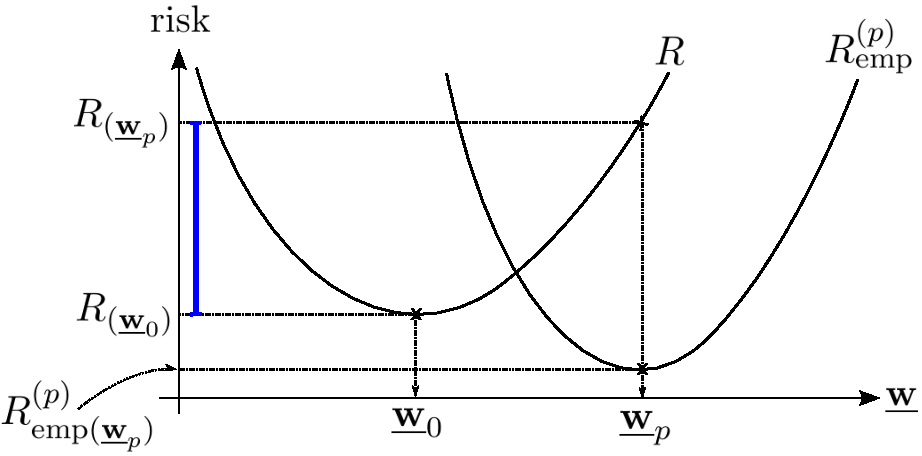
\includegraphics[width=9cm]{img/section2_fig1_question1}
	\end{center}
	\begin{enumerate}\setcounter{enumi}{1}
		\item {\textbf finite samples:} deviation from the optimal model
			\vspace{-2mm}
			$$
				P\bigg\{ {%\color{question1} 
				\Big| R_{(\vec w_p)} - R_{(\vec w_0)} \Big| }
					> \Big(\smallfrac{G^\Lambda_{(2p)} 
						- \ln \frac{\epsilon}{8}}{p} \Big)^\frac{1}{2}
					+ \Big(-\smallfrac{\ln \frac{\epsilon}{2}}{2p} 
						\Big)^\frac{1}{2} + \smallfrac{1}{p}
				\bigg\} < \epsilon
			$$
			\vspace{-4mm}
			\iitem{ finite $\dvc$: increased sample size $p$ 
				$\Rightarrow$ reduction of the bound}
	\end{enumerate}
\end{frame}

\begin{frame}\frametitle{The solution to learning problem 3} 
	\begin{center}
		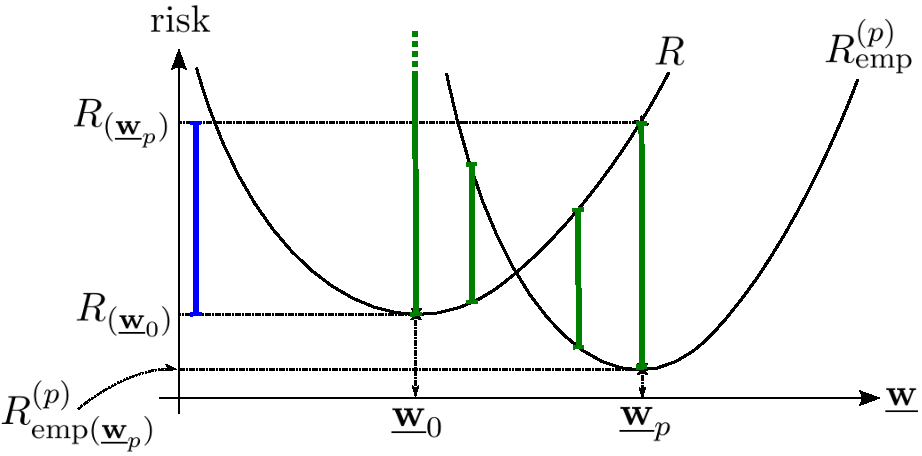
\includegraphics[width=9cm]{img/section2_fig1_question2_lessw}
	\end{center}
	\begin{enumerate}\setcounter{enumi}{2}
		\item {\textbf finite samples:} bound on the generalization error
			\vspace{-2mm}
			$$
				P\bigg\{ \sup\limits_{\vec w \in \Lambda}
					{%\color{question2} 
						\Big|R_{(\vec w)} - R^{(p)}_{\text{emp}(\vec w)}\Big| 
					} > \eta
				\bigg\} < 4 \exp\Big( G^\Lambda_{(2p)} 
					- p \big( \eta - \smallfrac{1}{p} \big)^2 \Big)
			$$
			\vspace{-4mm}
			\iitem{ bound non-trivial only if $G^\Lambda_{(2p)}$ 
				is sub-linear in $p$}
	\end{enumerate}
\end{frame}
